\documentclass[11pt,compress,t,notes=noshow, xcolor=table]{beamer}
\usepackage[]{graphicx}\usepackage[]{color}
% maxwidth is the original width if it is less than linewidth
% otherwise use linewidth (to make sure the graphics do not exceed the margin)
\makeatletter
\def\maxwidth{ %
  \ifdim\Gin@nat@width>\linewidth
    \linewidth
  \else
    \Gin@nat@width
  \fi
}
\makeatother

\definecolor{fgcolor}{rgb}{0.345, 0.345, 0.345}
\newcommand{\hlnum}[1]{\textcolor[rgb]{0.686,0.059,0.569}{#1}}%
\newcommand{\hlstr}[1]{\textcolor[rgb]{0.192,0.494,0.8}{#1}}%
\newcommand{\hlcom}[1]{\textcolor[rgb]{0.678,0.584,0.686}{\textit{#1}}}%
\newcommand{\hlopt}[1]{\textcolor[rgb]{0,0,0}{#1}}%
\newcommand{\hlstd}[1]{\textcolor[rgb]{0.345,0.345,0.345}{#1}}%
\newcommand{\hlkwa}[1]{\textcolor[rgb]{0.161,0.373,0.58}{\textbf{#1}}}%
\newcommand{\hlkwb}[1]{\textcolor[rgb]{0.69,0.353,0.396}{#1}}%
\newcommand{\hlkwc}[1]{\textcolor[rgb]{0.333,0.667,0.333}{#1}}%
\newcommand{\hlkwd}[1]{\textcolor[rgb]{0.737,0.353,0.396}{\textbf{#1}}}%
\let\hlipl\hlkwb

\usepackage{framed}
\makeatletter
\newenvironment{kframe}{%
 \def\at@end@of@kframe{}%
 \ifinner\ifhmode%
  \def\at@end@of@kframe{\end{minipage}}%
  \begin{minipage}{\columnwidth}%
 \fi\fi%
 \def\FrameCommand##1{\hskip\@totalleftmargin \hskip-\fboxsep
 \colorbox{shadecolor}{##1}\hskip-\fboxsep
     % There is no \\@totalrightmargin, so:
     \hskip-\linewidth \hskip-\@totalleftmargin \hskip\columnwidth}%
 \MakeFramed {\advance\hsize-\width
   \@totalleftmargin\z@ \linewidth\hsize
   \@setminipage}}%
 {\par\unskip\endMakeFramed%
 \at@end@of@kframe}
\makeatother

\definecolor{shadecolor}{rgb}{.97, .97, .97}
\definecolor{messagecolor}{rgb}{0, 0, 0}
\definecolor{warningcolor}{rgb}{1, 0, 1}
\definecolor{errorcolor}{rgb}{1, 0, 0}
\newenvironment{knitrout}{}{} % an empty environment to be redefined in TeX

\usepackage{alltt}
\newcommand{\SweaveOpts}[1]{}  % do not interfere with LaTeX
\newcommand{\SweaveInput}[1]{} % because they are not real TeX commands
\newcommand{\Sexpr}[1]{}       % will only be parsed by R



\usepackage[english]{babel}
\usepackage[utf8]{inputenc}

\usepackage{dsfont}
\usepackage{verbatim}
\usepackage{amsmath}
\usepackage{amsfonts}
\usepackage{bm}
\usepackage{csquotes}
\usepackage{multirow}
\usepackage{longtable}
\usepackage{booktabs}
\usepackage{enumerate}
\usepackage[absolute,overlay]{textpos}
\usepackage{psfrag}
\usepackage{algorithm}
\usepackage{algpseudocode}
\usepackage{eqnarray}
\usepackage{arydshln}
\usepackage{tabularx}
\usepackage{placeins}
\usepackage{tikz}
\usepackage{setspace}
\usepackage{colortbl}
\usepackage{mathtools}
\usepackage{wrapfig}
\usepackage{bm}
\usetikzlibrary{shapes,arrows,automata,positioning,calc,chains,trees, shadows}
\tikzset{
  %Define standard arrow tip
  >=stealth',
  %Define style for boxes
  punkt/.style={
    rectangle,
    rounded corners,
    draw=black, very thick,
    text width=6.5em,
    minimum height=2em,
    text centered},
  % Define arrow style
  pil/.style={
    ->,
    thick,
    shorten <=2pt,
    shorten >=2pt,}
}
\usepackage{subfig}


% Defines macros and environments
% basic latex stuff
\newcommand{\pkg}[1]{{\fontseries{b}\selectfont #1}} % fontstyle for R packages

% Often used in exercise Rnw files, still relevant?
\newcommand{\lz}{\vspace{0.5cm}} % vertical space
\newcommand{\dlz}{\vspace{1cm}}  % double vertical space

% Unused and about to be deleted
\newcommand{\oneliner}[1] % Oneliner for important statements
{\begin{block}{}\begin{center}\begin{Large}#1\end{Large}\end{center}\end{block}}


%--------------------%
%  New environments  %
%--------------------%

 % Frame with breaks and verbatim // this is used very often
\newenvironment{vbframe}
{
\begin{frame}[containsverbatim,allowframebreaks]
}
{
\end{frame}
}

% Frame with verbatim without breaks (to avoid numbering one slided frames)
% This is not used anywhere but I can see it being useful
\newenvironment{vframe}
{
\begin{frame}[containsverbatim]
}
{
\end{frame}
}

% Itemize block
\newenvironment{blocki}[1]
{
\begin{block}{#1}\begin{itemize}
}
{
\end{itemize}\end{block}
}

%--------------%
%  Citebutton  %
%--------------%
% Example usage (from slides-cart-discussion.tex)
% \citebutton{Breiman, 1984}{https://www.taylorfrancis.com/books/mono/10.1201/9781315139470/classification-regression-trees-leo-breiman}
\newcommand{\citebutton}[2]{%
\NoCaseChange{\resizebox{!}{9pt}{\protect\beamergotobutton{\href{#2}{#1}}}}%
}

% textcolor that works in mathmode
% https://tex.stackexchange.com/a/261480
% Used e.g. in forests/slides-forests-bagging.tex
% [...] \textcolor{blue}{\tfrac{1}{M}\sum^M_{m} [...]
\makeatletter
\renewcommand*{\@textcolor}[3]{%
  \protect\leavevmode
  \begingroup
    \color#1{#2}#3%
  \endgroup
}
\makeatother

% % basic latex stuff
\newcommand{\pkg}[1]{{\fontseries{b}\selectfont #1}} % fontstyle for R packages

% Often used in exercise Rnw files, still relevant?
\newcommand{\lz}{\vspace{0.5cm}} % vertical space
\newcommand{\dlz}{\vspace{1cm}}  % double vertical space

% Unused and about to be deleted
\newcommand{\oneliner}[1] % Oneliner for important statements
{\begin{block}{}\begin{center}\begin{Large}#1\end{Large}\end{center}\end{block}}


%--------------------%
%  New environments  %
%--------------------%

 % Frame with breaks and verbatim // this is used very often
\newenvironment{vbframe}
{
\begin{frame}[containsverbatim,allowframebreaks]
}
{
\end{frame}
}

% Frame with verbatim without breaks (to avoid numbering one slided frames)
% This is not used anywhere but I can see it being useful
\newenvironment{vframe}
{
\begin{frame}[containsverbatim]
}
{
\end{frame}
}

% Itemize block
\newenvironment{blocki}[1]
{
\begin{block}{#1}\begin{itemize}
}
{
\end{itemize}\end{block}
}

%--------------%
%  Citebutton  %
%--------------%
% Example usage (from slides-cart-discussion.tex)
% \citebutton{Breiman, 1984}{https://www.taylorfrancis.com/books/mono/10.1201/9781315139470/classification-regression-trees-leo-breiman}
\newcommand{\citebutton}[2]{%
\NoCaseChange{\resizebox{!}{9pt}{\protect\beamergotobutton{\href{#2}{#1}}}}%
}

% textcolor that works in mathmode
% https://tex.stackexchange.com/a/261480
% Used e.g. in forests/slides-forests-bagging.tex
% [...] \textcolor{blue}{\tfrac{1}{M}\sum^M_{m} [...]
\makeatletter
\renewcommand*{\@textcolor}[3]{%
  \protect\leavevmode
  \begingroup
    \color#1{#2}#3%
  \endgroup
}
\makeatother


%\usetheme{lmu-lecture}
\usepackage{../../style/lmu-lecture}

\let\code=\texttt
\let\proglang=\textsf

\setkeys{Gin}{width=0.9\textwidth}

\title{Introduction to Machine Learning}
% \author{Bernd Bischl, Christoph Molnar, Daniel Schalk, Fabian Scheipl}
\institute{\href{https://compstat-lmu.github.io/lecture_i2ml/}{compstat-lmu.github.io/lecture\_i2ml}}
\date{}

\setbeamertemplate{frametitle}{\expandafter\uppercase\expandafter\insertframetitle}



\begin{document}


% This file loads R packages, configures knitr options and sets preamble.Rnw as parent file
% IF YOU MODIFY THIS, PLZ ALSO MODIFY setup.Rmd ACCORDINGLY...








%! includes: evaluation-measures-classification

\lecturechapter{Evaluation: Measures for Binary Classification: ROC Measures}
\lecture{Introduction to Machine Learning}

\begin{vbframe}{Imbalanced Binary Labels}

\begin{center}
% FIGURE SOURCE: https://docs.google.com/drawings/d/1WERS9WXwS4zla86fk6ESQkskNN1WZMI1YCPprnp0Ew0/edit?usp=sharing
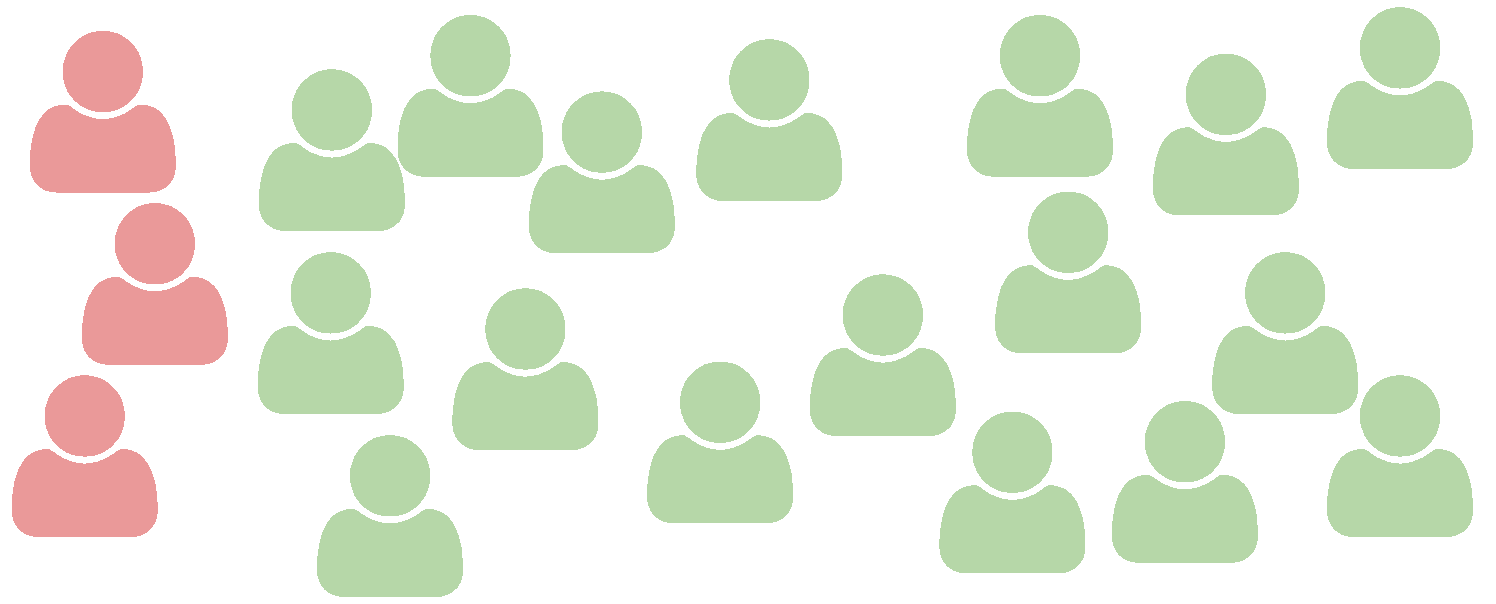
\includegraphics[width=.9\textwidth]{figure_man/imbalanced.pdf}\\
Classify all as \enquote{no disease} (green) $\rightarrow$ high accuracy.

\lz

\textbf{Accuracy Paradox}
\end{center}

\end{vbframe}


\begin{vbframe}{Imbalanced Costs}

\begin{center}
% FIGURE SOURCE: https://docs.google.com/drawings/d/1GlmMqzpeNHU_rtPFIrJMlY9Iz6XexvHEwTl3dNYKyQU/edit?usp=sharing
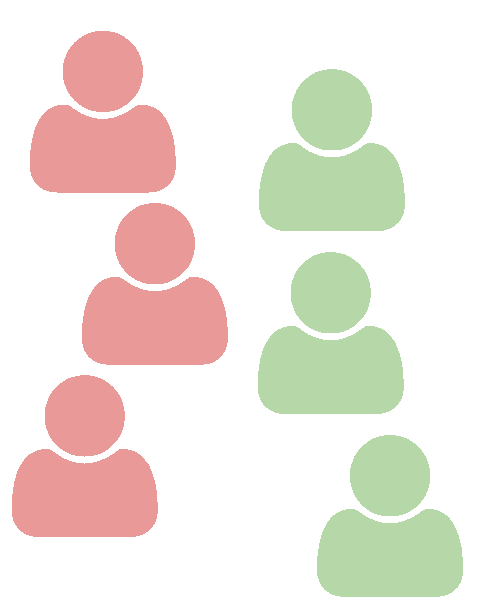
\includegraphics[width=.3\textwidth]{figure_man/imbalanced-costs.pdf}\\
Classify incorrectly as \enquote{no disease} $\rightarrow$ very high cost

\end{center}

\end{vbframe}

% \begin{vbframe}{Imbalanced Binary Labels}
% \begin{itemize}
%   \item Consider a binary classifier for diagnosing a serious medical condition
%   \item Here, label distribution is often \textbf{imbalanced}, i.e, not many people have the disease
%   \item Evaluating with error rate for imbalanced labels is often inappropriate
%   \item Assume that only 0.5\,\% of 1000 patients have the disease
%   \item Always returning "no disease" has an error rate of 0.5\,\%, which sounds good
%   \item However, this sends all sick patients home, which is the worst possible system, even classifying everyone as "sick" might be better, depending on what happens next
%   \item This problem is sometimes known as the \textbf{accuracy paradox}
% \end{itemize}
% \end{vbframe}
% 
% \begin{vbframe}{Binary Classifiers and Costs}
% \begin{itemize}
%   \item Another point of view is imbalanced costs
%   \item In our example, classifying a sick patient as healthy, should incur a much higher loss then classifying a healthy patient as sick
%   \item The costs depend a lot on what happens next: We can likely assume that our system is some type of screening filter,
%     often the next step after labeling someone as "sick" might be a more invasive, expensive, but more reliable test for the disease
%   \item Erroneously subjecting someone to that second step is not good (psychologically, economically, or because the second test might introduce
%     medical risks), but sending someone home to get worse or die seems much worse
%   \item Such a situation not only arises under label imbalance, but also when labels are maybe balanced but costs differ
%   \item We could see this as imbalanced costs of misclassification, rather than imbalanced labels; both situations are tightly connected
% \end{itemize}
% \end{vbframe}
% 
% \begin{vbframe}{Binary Classifiers and Costs}
% \begin{itemize}
%   \item Problem is: If we could specify costs precisely, we could evaluate against them, we might even optimize our model for them
%   \item This important subfield of ML is called \textbf{cost-sensitive learning}, which we will not cover in this lecture unit
%   \item Unfortunately, users often have a notoriously hard time to come up with precise cost numbers in imbalanced scenarios
%   \item Evaluating "from different perspectives", with multiple metrics, often helps, especially to get a first impression
%     of the quality of the system
% \end{itemize}
% \end{vbframe}
% 

% 
% 
% \begin{vbframe}{Confusion Matrix and ROC Metrics}
% \begin{itemize}
%   \item From now on, we call one class "positive", one "negative" and their respective sizes
%     $n_+$ and $n_-$
%   \item The positive class is the more important, often smaller one
%   \item We represent all predictions in a confusion matrix and count correct and incorrect class assignments
%   \item False Positive means: We assigned "positive", but were wrong
% \end{itemize}
% % FIGURE SOURCE: No source
% 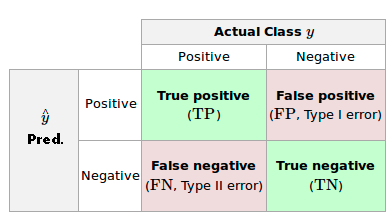
\includegraphics[width=0.7\textwidth]{figure_man/roc-confmatrix1.png}
% \end{vbframe}


\begin{vbframe}{Confusion Matrix}

\begin{center}
\small
\renewcommand{\arraystretch}{1.5}
\begin{tabular}{cc||cc}
    & & \multicolumn{2}{c}{\bfseries True Class $y$}  \\
    & & $+$ & $-$  \\ 
    \hline \hline
    \bfseries Pred.     & $+$ & TP & FP\\
              $\hat{y}$ & $-$ & FN & TN\\ 
\end{tabular}
\renewcommand{\arraystretch}{1}
\end{center}

\begin{itemize}
  \item $+$: \enquote{positive} class
  \item $-$: \enquote{negative} class
  \item $n_+$: number of observations in $+$
  \item $n_-$: number of observations in $-$
\end{itemize}
\end{vbframe}


\begin{vbframe}{Labels: ROC Metrics}
From the confusion matrix (binary case), we can calculate "ROC" metrics.

% % FIGURE SOURCE: No source
% 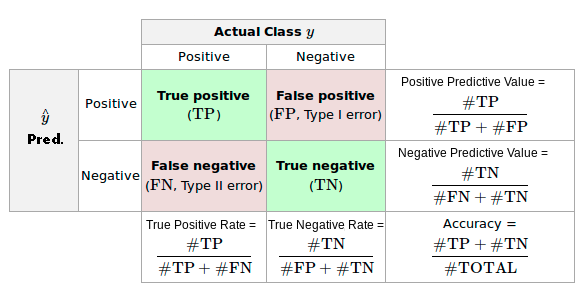
\includegraphics[width=0.7\textwidth]{figure_man/roc-confmatrix2.png}

% \begin{center}
% \small
% \begin{tabular}{cc|>{\centering\arraybackslash}p{7em}>{\centering\arraybackslash}p{8em}|>{\centering\arraybackslash}p{8em}}
%     & & \multicolumn{2}{c}{\bfseries True Class $y$} & \\
%     & & $+$ & $-$ & \\
%     \hline
%     \bfseries Pred.     & $+$ & True Positive (TP)  & False Positive (FP) & Positive Predictive Value (PPV) = $\frac{\text{TP}}{\text{TP} + \text{FP}}$\\
%               $\hat{y}$ & $-$ & False Negative (FN) & True Negative (TN) & Negative Predictive Value (NPV) = $\frac{\text{TN}}{\text{FN} + \text{TN}}$\\
%     \hline
%     & & TPR = $\frac{\text{TP}}{\text{TP} + \text{FN}}$ & TNR = $\frac{\text{TN}}{\text{FP} + \text{TN}}$ & Accuracy = $\frac{\text{TP}+ \text{TN}}{\text{TOTAL}}$
% \end{tabular}
% \end{center}

\begin{center}
\small
\renewcommand{\arraystretch}{1.5}
\begin{tabular}{cc||cc|c}
    & & \multicolumn{2}{c|}{\bfseries True Class $y$} & \\
    & & $+$ & $-$ & \\ 
    \hline \hline
    \bfseries Pred.     & $+$ & TP & FP & PPV = $\frac{\text{TP}}{\text{TP} + \text{FP}}$\\
              $\hat{y}$ & $-$ & FN & TN & NPV = $\frac{\text{TN}}{\text{FN} + \text{TN}}$\\
    \hline
    & & TPR = $\frac{\text{TP}}{\text{TP} + \text{FN}}$ & TNR = $\frac{\text{TN}}{\text{FP} + \text{TN}}$ & Accuracy = $\frac{\text{TP}+ \text{TN}}{\text{TOTAL}}$
\end{tabular}
\renewcommand{\arraystretch}{1}
\end{center}

\begin{itemize}
  \item True Positive Rate: How many of the true 1s did we predict as 1?
  \item True Negative Rate: How many of the true 0s did we predict as 0?
  \item Positive Predictive Value: If we predict 1 how likely is it a true 1?
  \item Negative Predictive Value: If we predict 0 how likely is it a true 0?
\end{itemize}
\end{vbframe}


\begin{frame}{History ROC}
ROC = receiver operating characteristics

\lz

Initially developed by electrical engineers and radar engineers during World War II for detecting enemy objects in battlefields. 

\begin{center}
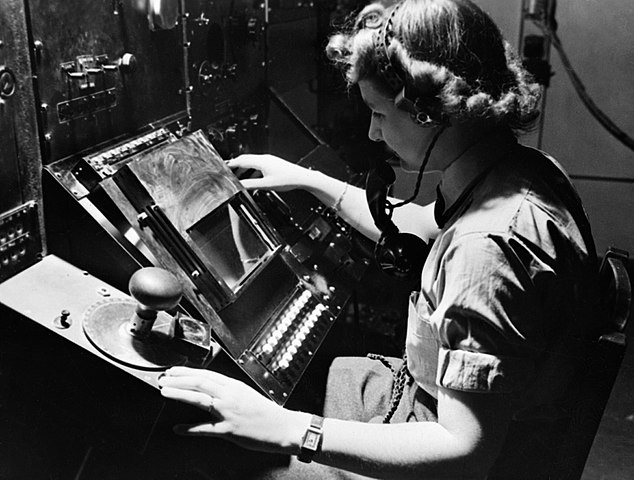
\includegraphics[width=.4\textwidth]{figure_man/receiver_operator.jpg}
{\tiny \url{http://media.iwm.org.uk/iwm/mediaLib//39/media-39665/large.jpg}}
\end{center}

Still has the funny name.
\end{frame}


\begin{vbframe}{Labels: ROC}
Example
\begin{center}
  % FIGURE SOURCE: No source
  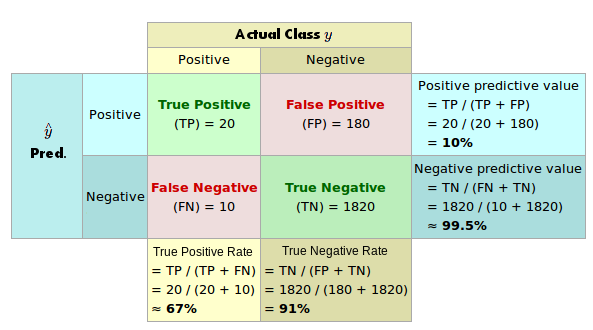
\includegraphics[width=\textwidth]{figure_man/roc-confmatrix-example.png}
\end{center}

\end{vbframe}

\begin{vbframe}{More metrics and alternative terminology}

Unfortunately, for many concepts in ROC, 2-3 different terms exist.

\begin{center}
% FIGURE SOURCE: https://en.wikipedia.org/wiki/F1_score#Diagnostic_testing
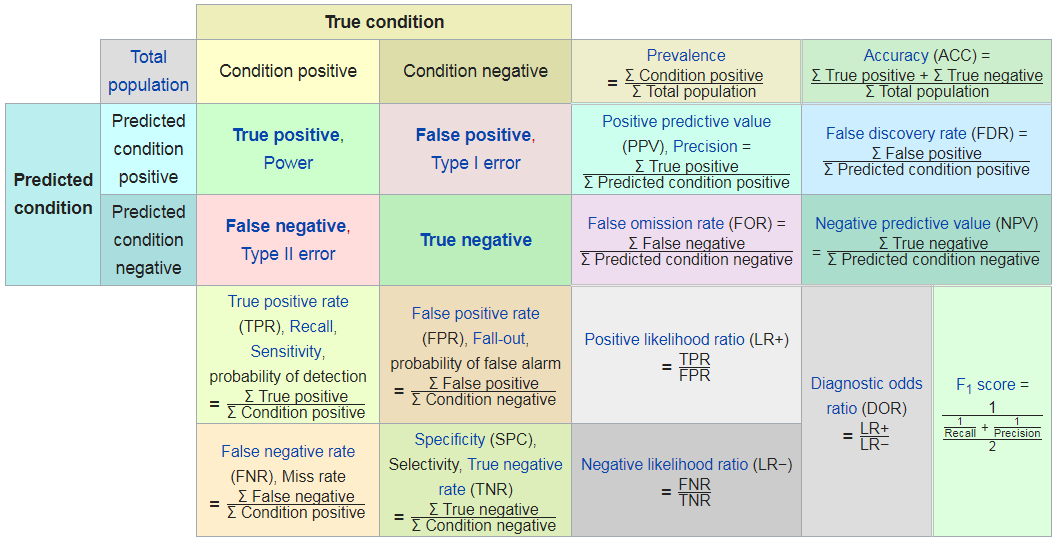
\includegraphics[width=0.95\textwidth]{figure_man/roc-confmatrix-allterms.png}
\end{center}
\href{https://en.wikipedia.org/wiki/F1_score#Diagnostic_testing}{\beamergotobutton{Clickable version/picture source}} $\phantom{blablabla}$
\href{https://upload.wikimedia.org/wikipedia/commons/0/0e/DiagnosticTesting_Diagram.svg}{\beamergotobutton{Interactive diagram}}
\end{vbframe}


\begin{vbframe}{Labels: $F_1$-Measure}

% \begin{itemize}
%   \item It is difficult to achieve a high \textit{Positive Predictive Value} and high \textit{True Positive Rate} simultaneously.
%   \item A classifier that predicts more "positives" will tend to be more sensitive (higher TPR), but it will also tend to give more false positives (lower TNR, lower PPV).
%   \item A classifier that predicts more "negatives" will tend to be more precise (higher PPV), but it will also produce more false negatives (lower TPR).
% \end{itemize}

\lz
A measure that balances two conflicting goals\\[.5em]
\begin{enumerate}
 \item Maximising Positive Predictive Value
 \item Maximising True Positive Rate\\[.5em]
\end{enumerate}
is the harmonic mean of PPV and TPR:
$$F_1 = 2 \cfrac{PPV \cdot TPR}{PPV + TPR}$$

\lz \lz
Note: still doesn’t account for the number of true negatives.
\end{vbframe}

\begin{vbframe}{Labels: $F_1$-Measure}
Tabulated $F_1$-Score for different TPR (rows) and PPV (cols) combinations. 
\begin{knitrout}\scriptsize
\definecolor{shadecolor}{rgb}{0.969, 0.969, 0.969}\color{fgcolor}\begin{kframe}
\begin{verbatim}
    0.0  0.2  0.4  0.6  0.8  1.0
0.0   0 0.00 0.00 0.00 0.00 0.00
0.2   0 0.20 0.27 0.30 0.32 0.33
0.4   0 0.27 0.40 0.48 0.53 0.57
0.6   0 0.30 0.48 0.60 0.69 0.75
0.8   0 0.32 0.53 0.69 0.80 0.89
1.0   0 0.33 0.57 0.75 0.89 1.00
\end{verbatim}
\end{kframe}
\end{knitrout}
$\rightarrow$ Tends more towards the lower of the 2 combined values.


\begin{itemize}
  \item $TPR = 0$ or $PPV=0$ $\Rightarrow$ $F_1$ of 0
  \item Predicting always "neg": $F_1 = 0$
  \item Predicting always "pos": $F_1 = 2 PPV / (PPV + 1) = 2 n_+ / (n_+ + n)$,\\ 
  which will be rather small, if the size of the positive class $n_+$ is small.
\end{itemize}


\end{vbframe}

\endlecture

\end{document}
